\subsubsection{Presentacion de estudiente para su curso}

{\textbf {Resumen:}}
Un alumno de enseñanza media tiene que hacer una presentación sobre un tema histórico local, el recuerda que hay informacion de esto en el museo pero no puede ir por cuarentena (COVID), a su vez recuerda que en la aplicación “museo en casa” tiene esa pieza en su colección, días después el estudiante presenta sin problemas ya que pudo obtener la información necesaria para esta desde la información entregada por la aplicación.

{\textbf {Actores:}}
Estudiante.

{\textbf {Propósito:}}
Mostrar usos prácticos de la aplicación que no tengan una relación directa con su parte lúdica.

{\textbf {Referencias cruzadas:}}
R1.1, R1.2, R2.7,R2.8, R5.3, R6.1, R6.5

\paragraph{Caso de Uso Esencial}

\begin{longtable}{|p{5cm}|p{8cm}|}
\hline 
Acción actores & Respuesta del sistema \\ 
\hline 
El alumno abre la aplicación y entra al menu de piezas & La aplicación muestra un listado de las piezas. \\ 
\hline
El alumno ocupa el buscador de pieza para encontrar la que necesita en su presentación. & La aplicación solo muestra la información relacionada a lo ingresado por el usuario. \\ 
\hline 
El jugador encuentra, la pieza que busca y la clickea. & El sistema abre un panel con la información de la pieza independiente si esta la tiene en su colección pero no las opciones lúdicas. \\ 
\hline 
El usuario utiliza la aplicación como fuente de datos para su presentación y no se preocupa de no disponer de las opciones lúdicas ya que no son necesarias. & --- \\ 
\hline 
\caption{Tabla de Caso de Uso Esencial 1.4}
\label{tab24}
\end{longtable}

\paragraph{Diagrama de Caso de Uso}

\begin{figure}[H]
\centerline{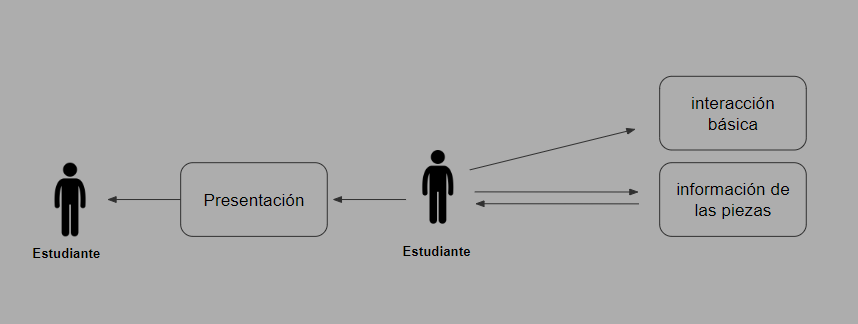
\includegraphics[width=15cm]{imgs/CasoUso_4.PNG}}
\caption{Diagrama Caso 1.4}
\label{fig_4_1}
\end{figure}

\paragraph{Modelo Conceptual}

\begin{figure}[H]
\centerline{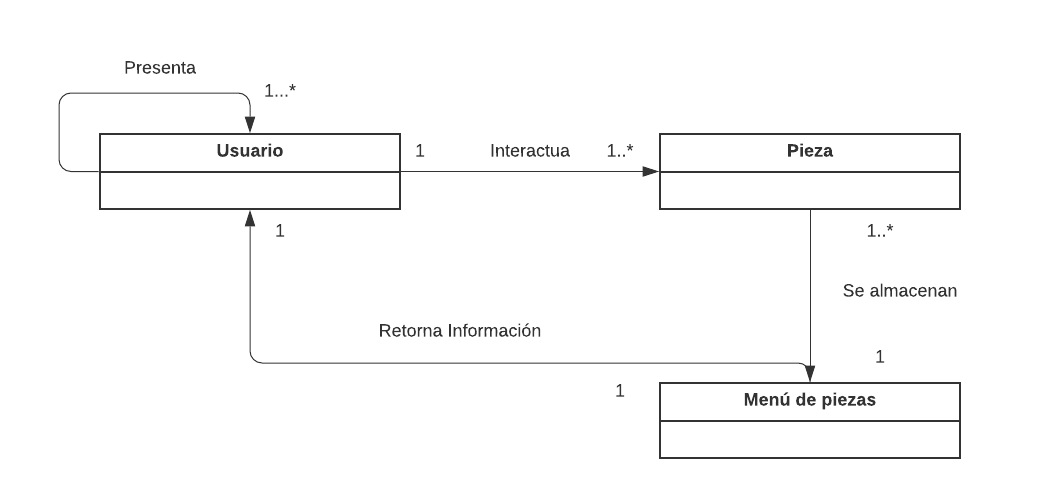
\includegraphics[width=15cm]{imgs/ModeloConceptualCaso_4_3.png}}
\caption{Modelo Conceptual Caso 1.4}
\label{fig_4_2}
\end{figure}


\paragraph{Diagrama de Secuencia o Colaboración}

\begin{figure}[H]
\centerline{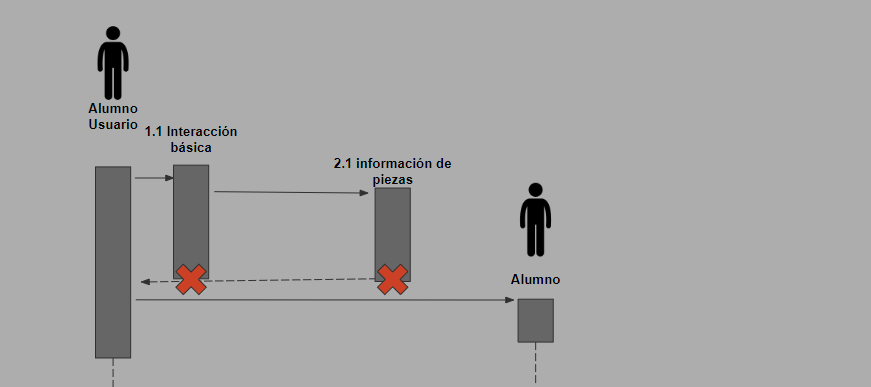
\includegraphics[width=15cm]{imgs/CasoUso_4_2.PNG}}
\caption{Diagrama de Secuencia Caso 1.4}
\label{fig_4_3}
\end{figure}

\paragraph{Priorización}
{\textbf {Tipo:}}
Deseable.